\documentclass[10pt,journal,compsoc]{IEEEtran}

\usepackage{algorithmic}
\usepackage{array}
 \usepackage[nocompress]{cite}
 \usepackage{color}
\usepackage{listings}
\usepackage[caption=false,font=normalsize,labelfont=sf,textfont=sf]{subfig}
\usepackage{stfloats}
\usepackage{url}


\usepackage[pdftex]{graphicx}
\graphicspath{{./figs}}
\DeclareGraphicsExtensions{.pdf,.jpeg,.png}


% *** MATH PACKAGES ***
\usepackage{amsmath}
\interdisplaylinepenalty=2500

% correct bad hyphenation here
\hyphenation{op-tical net-works semi-conduc-tor}


\begin{document}

% title
\title{Reproducible Workflow on a Public Cloud for Computational Fluid Dynamics}
% author names and affiliations
\author{Olivier Mesnard, Lorena A. Barba
\IEEEcompsocitemizethanks{\IEEEcompsocthanksitem Mechanical and Aerospace Engineering,
the George Washington University, Washington, DC 20052.\protect\\
% note need leading \protect in front of \\ to get a newline within \thanks as
% \\ is fragile and will error, could use \hfil\break instead.
E-mail: mesnardo@gwu.edu
\IEEEcompsocthanksitem Email: labarba@gwu.edu}% <-this % stops an unwanted space
%\thanks{Manuscript submitted 2019}
}

\IEEEtitleabstractindextext{%
\begin{abstract}
In a new effort to make our research transparent and reproducible by others, we have developed a workflow to run computational studies on a public cloud. It uses Docker containers to create an image of the application software stack. We also adopt several tools that facilitate creating and managing virtual machines with compute nodes and submitting jobs to these nodes. The configuration files for these tools are part of an expanded "reproducibility package" that includes workflow definitions for cloud computing, in addition to input files and instructions. This facilitates re-creating the cloud environment to re-un the simulations under the same conditions.
\end{abstract}
}

% make the title area
\maketitle

\IEEEraisesectionheading{\section{Introduction}\label{sec:introduction}}

\section{Reproducible Workflow}\label{sec:workflow}

CFD publications often lack details about external libraries used along with the main computational code.
We have learned the hard way how different versions of the same external library can alter the numerical results and even the scientific findings of a computational study\cite{mesnard_barba_2017}.
To overcome the so-called ``dependency hell'' and facilitate reproducibility, we use Docker to locally create an image of our computational application.
Container technology facilitates share build images of the full software stack that is used to produce scientific results.
The process of building an image using Docker begins with writing an ASCII file, called a Dockerfile, that contains Docker keywords and system commands for building multi-layered software stack.
Once the image is build locally, we push it to a public registry (e.g., DockerHub).
Everyone can now pull the application image and create a container to run the application in a faithfully reproduced local environment.
We aim to move the final stage of this workflow (creating a container) to a public cloud provider such as Microsoft Azure.

To run computational jobs on Microsoft Azure, we use several tools that facilitate creating and managing virtual machines with compute nodes and submitting jobs to those nodes.
\ref{fig:cloud_workflow} shows a graphical representation of the workflow we adopted to run CFD simulations with an in-house software on Microsoft Azure.
We use a Microsoft Azure platform service called Azure Batch to run our in-house CFD software.
Azure Batch services leverages Microsoft Azure at no extra cost to relieve the user from manually creating, configuring, and managing a HPC-capable cluster of cloud nodes, including virtual machines, virtual networks, job and task scheduling infrastructure.
Azure Batch works with both embarrassingly parallel workloads and tightly-coupled MPI jobs (the latter being the case of our CFD software).
To use Azure Batch, the user needs to configure a workspace on Microsoft Azure by creating an Azure Batch account associated to an Azure Storage account (to upload and download simulation data).
This can be done either via the Azure Portal in a web browser or from a local terminal user the open-source tool Azure CLI.\footnote{Azure CLI (version 2.0.57): \url{https://github.com/Azure/azure-cli}}

To create computational nodes and submit container-based jobs to Azure Batch, we use the open-source command-line utility Batch Shipyard.\footnote{Batch Shipyard (version 3.6.1): https://github.com/Azure/batch-shipyard} Batch Shipyard reads user-written YAML configuration files to automatically create pools of compute nodes on Microsoft Azure and to submit jobs to those pools.
The Docker image of our CFD application is pulled from the (public or private) registry to the virtual machines when the pool is created.
Once the simulations are done (i.e., the job tasks are complete), we delete the jobs and the pool.
The output of the computation is now stored on a fileshare in our Azure Storage account and we can download the data to our local machine to perform additional post-processing steps.

Reproducible research requires authors to make their code and data available.
Thus, the Dockerfile and YAML configuration files should be made part of an extended reproducibility package that includes workflow instructions for cloud computing, in addition to other input files.
Such reproducibility package facilitates re-creating the cloud environment to run the simulations under the same conditions.

\begin{figure*}[!h]
    \centering
    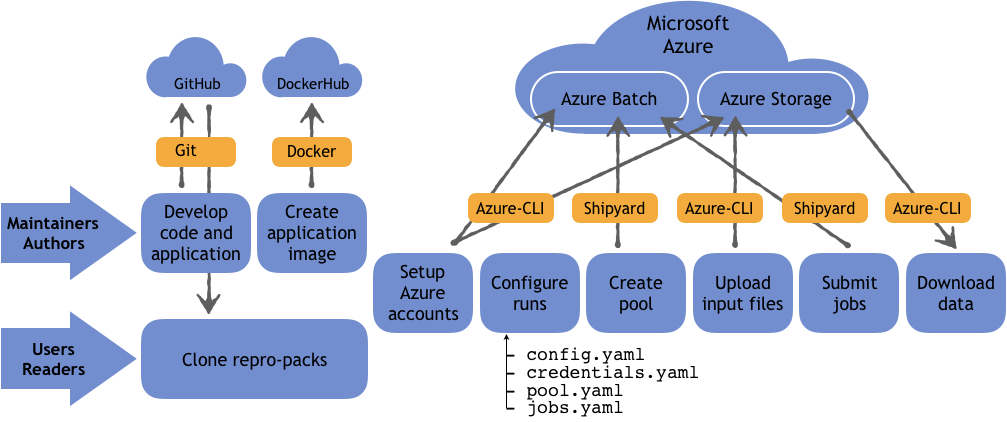
\includegraphics[width=14cm]{figures/cloud_workflow.png}
    \caption{Reproducible workflow on the public cloud provider Microsoft Azure.}
    \label{fig:cloud_workflow}
\end{figure*}

\begin{table*}[!h]
    \caption{NC series on Microsoft Azure. (Prices as of May 13, 2018.)}
    \label{tab:nc_series}
    \centering
    \begin{tabular}{cccccccc}
        Instance & cores & RAM & disk sizes & GPU & pay-as-you-go & 1-year reserved & 3-year reserved \\
        && (GiB) & (Gib) && (\$/hr) & (\$/hr) & (\$/hr) \\
        \hline
        NC6 & 6 & 56 & 340 & 1 x K80 & 0.90 & 0.574 & 0.40 \\
        NC12 & 12 & 112 & 680 & 2 x K80 & 1.80 & 1.147 & 0.80 \\
        NC24 & 24 & 224 & 1,440 & 4 x K80 & 3.60 & 2.294 & 1.599 \\
        NC24r\footnotemark & 24 & 224 & 1,440 & 4 x K80 & 3.96 & 2.523 & 1.758 \\
        \hline
    \end{tabular}
\end{table*}

\footnotetext{NC24r instances are RDMA (Remote Direct Access Memory) capable with InfiniBand network.}

\section{Results}\label{sec:results}

Thanks to a sponsorship ($\$20,000$ worth of cloud credits) from the Microsoft Azure for Research program,\footnote{Microsoft Azure for Research: \url{https://www.microsoft.com/en-us/research/academic-program/microsoft-azure-for-research/}} we ran three-dimensional CFD simulations of the flow around a gliding-snake model using our in-house research software PetIBM\cite{chuang_et_al_2018}.
Prior to that, we ran benchmarks to confirm we would get comparable performances between a local university-managed HPC cluster (Colonial One) and a public cloud platform such as Microsoft Azure.

\subsection{MPI Communication Benchmarks}\label{subsec:mpi_benchmarks}

We compared the MPI communication performances between Microsoft Azure and Colonial One using the micro-benchmarks from the Ohio State University\footnote{OSU Micro-Benchmarks (version 5.6): \url{http://mvapich.cse.ohio-state.edu/benchmarks/}} to perform point-to-point tests and evaluate the latency and bandwidth on the two clusters.
On Colonial One, we used two nodes (provide details of CPU) with InfiniBand network.
On Microsoft Azure, we used two NC24r instances (provide details of CPU) with RMDA over InfiniBand.
Figure \ref{fig:osu_benchmarks} report the latencies and bandwidths averaged over 5 repetitions.

\begin{figure}[!h]
    \centering
    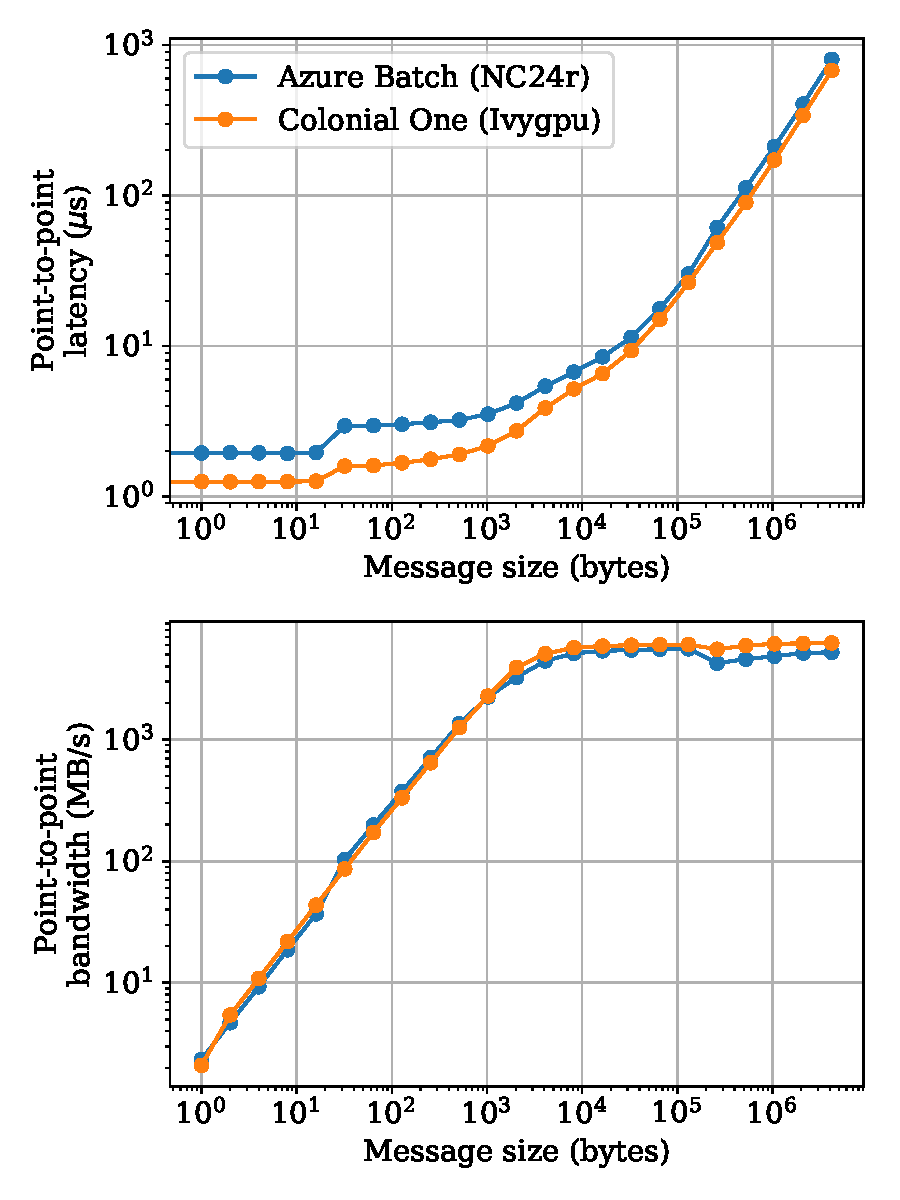
\includegraphics[width=8cm]{figures/osu_latency_bandwidth.pdf}
    \caption{Point-to-point latency (top) and bandwidth (bottom) obtained on Colonial One and on NC24r instances of Microsoft Azure.}
    \label{fig:osu_benchmarks}
\end{figure}

\subsection{Poisson Benchmarks}\label{subsec:poisson_benchmarks}

We compare the runtimes on the two platforms (Colonial One and Microsoft Azure) to solve a three-dimensional Poisson system (central differences on a uniform mesh) on CPUs and GPUs.
Figure \ref{fig:poisson_benchmarks} reports the runtimes (averaged over 5 repetitions) to solve the Poisson system.
On the CPU nodes, we perform strong scaling on a mesh size of $1000 \times 1000 \times 50$ cells using up to 8 nodes to solve the system with PETSc using a Conjugate Gradient method and a classical algebraic multigrid preconditioner from the package Hypre BoomerAMG.
On the nodes that feature GPU devices, we perform weak scaling starting with a mesh size of $500 \times 500 \times 25$ cells on a single node (using 12 CPU cores and 2 GPU devices); we double the mesh size as we double the number of nodes in the pool.
We use the NVIDIA AmgX library to solve the system with a Conjugate Gradient method and a classical algebraic multigrid preconditioner.
As the number of iterations to reach convergence increases with the size of the system, we normalize the runtimes by the number of iterations.

\begin{figure}[!h]
    \centering
    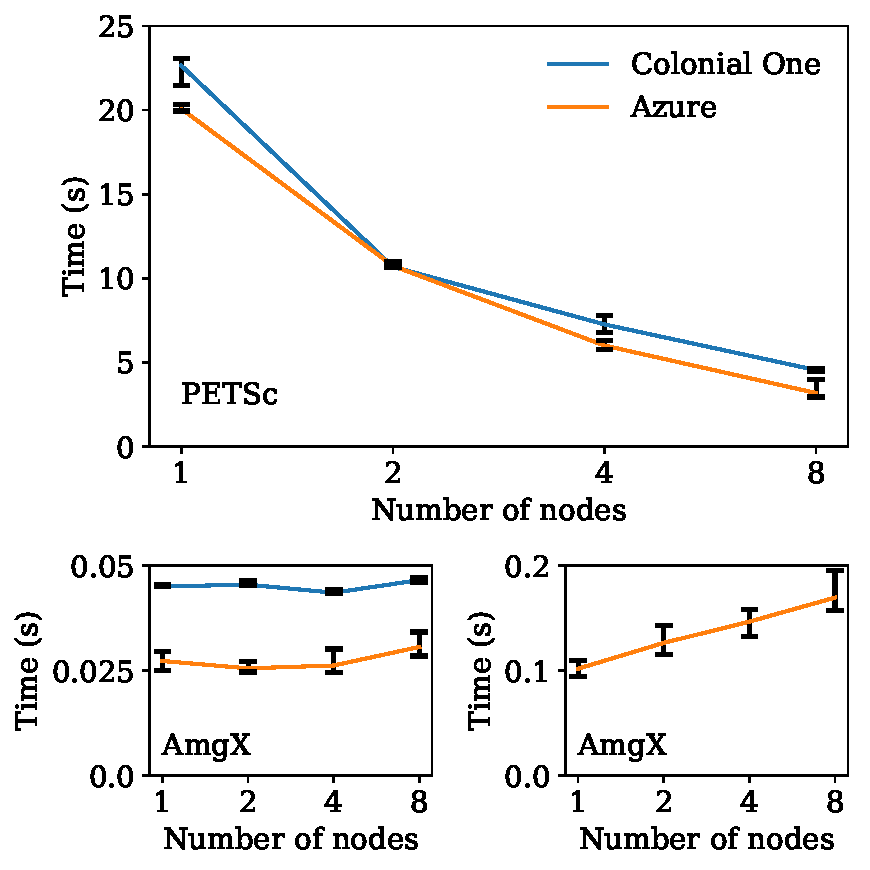
\includegraphics[width=8cm]{figures/poisson_time_vs_nodes.pdf}
    \caption{Runtimes to solve a Poisson system on Colonial One and on Microsoft Azure.}
    \label{fig:poisson_benchmarks}
\end{figure}

\subsection{Flow Around a Flying Snake Cross-Section}\label{subsec:snake}

Our research lab is interested in understanding the aerodynamics of flying animals using Computational Fluid Dynamics software.
One of our applications deals with the aerodynamics of a snake species, \textit{Chrysopelea Paradisi}, that lives in South-East Asia.
The arboreal reptile has the remarkable capacity to turn its entire body into a wing and glide over several meters\cite{socha_2011}.
The so-called flying snake jumps from tree branches, undulates in the air, and is able to produce lift by expanding its ribcage to flatten its ventral surface (morphing its normally circular cross-section into a triangular shape).

\begin{figure}[!h]
    \centering
    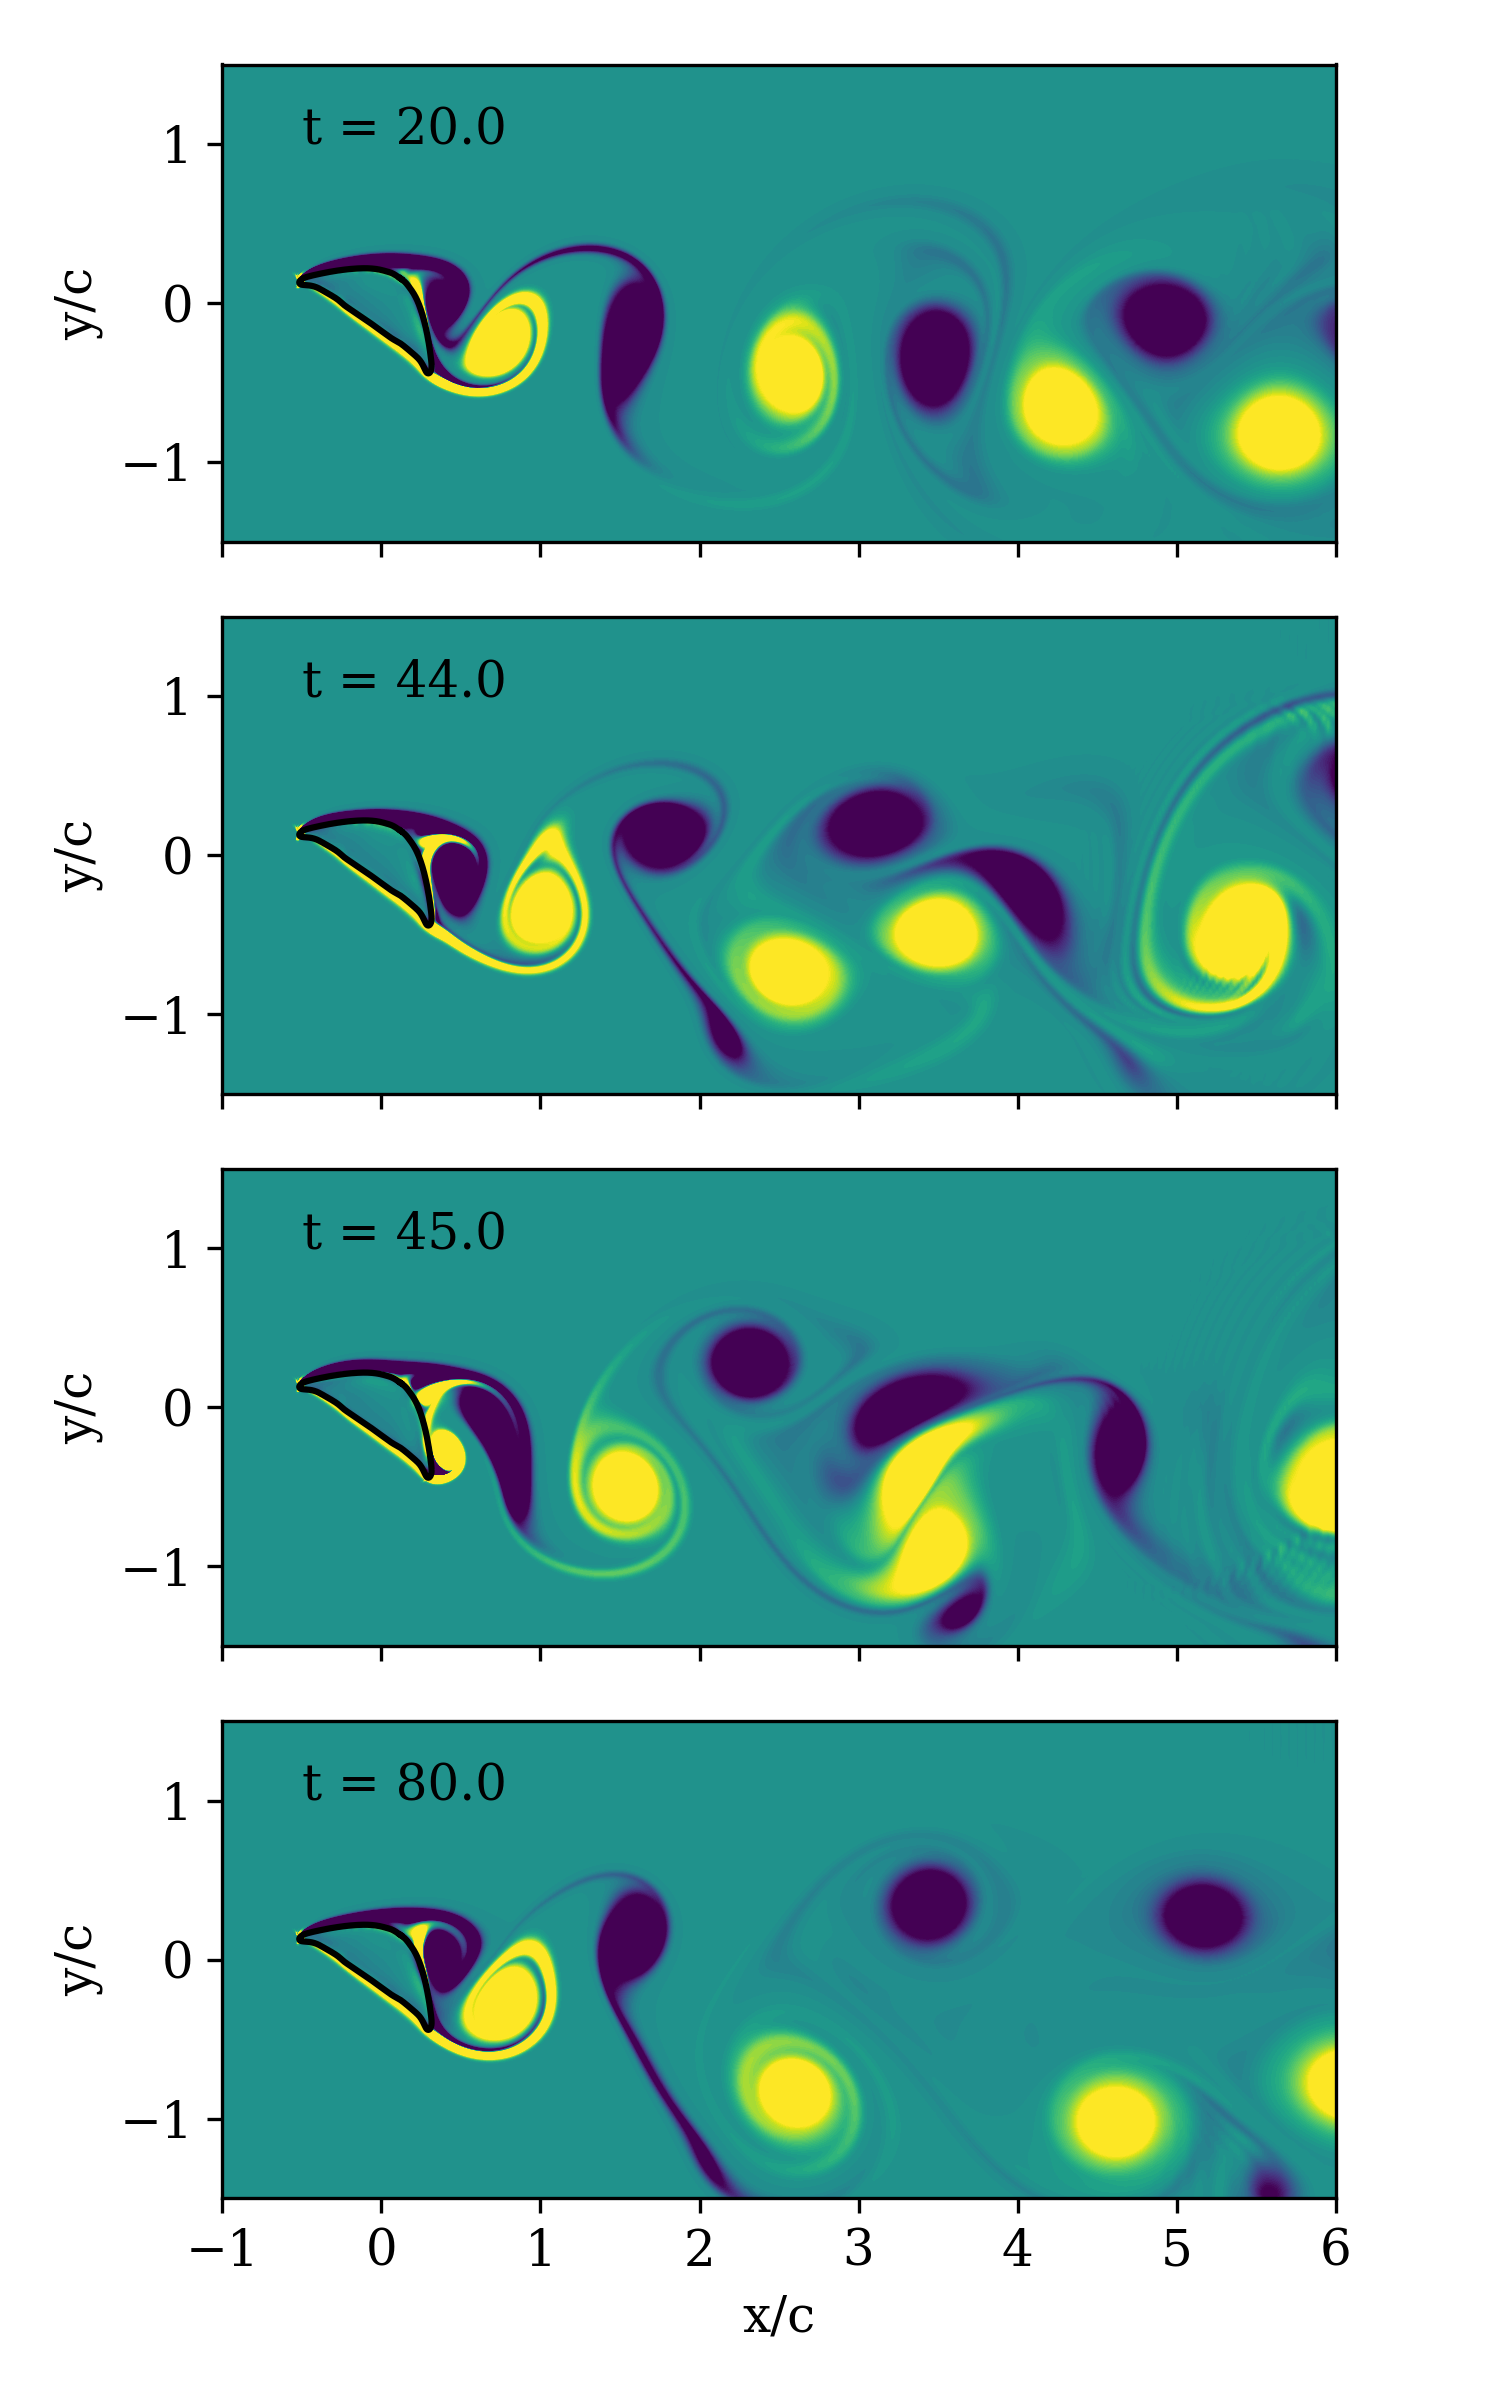
\includegraphics[width=8cm]{figures/wz_multi_contourf.png}
    \caption{Filled contour of the vorticity field ($-5 \leq w_z c / U_\infty \leq 5$) after $20$, $44$, $45$, and $80$ time units of flow simulation with PetIBM for the snake cross-section at a $35$-degree angle of attack and Reynolds number $2000$. Vortex merging events are responsible for the change in the wake signature and the drop in the mean value of the lift coefficient.}
    \label{fig:wz_2d}
\end{figure}

\begin{figure}[!h]
    \centering
    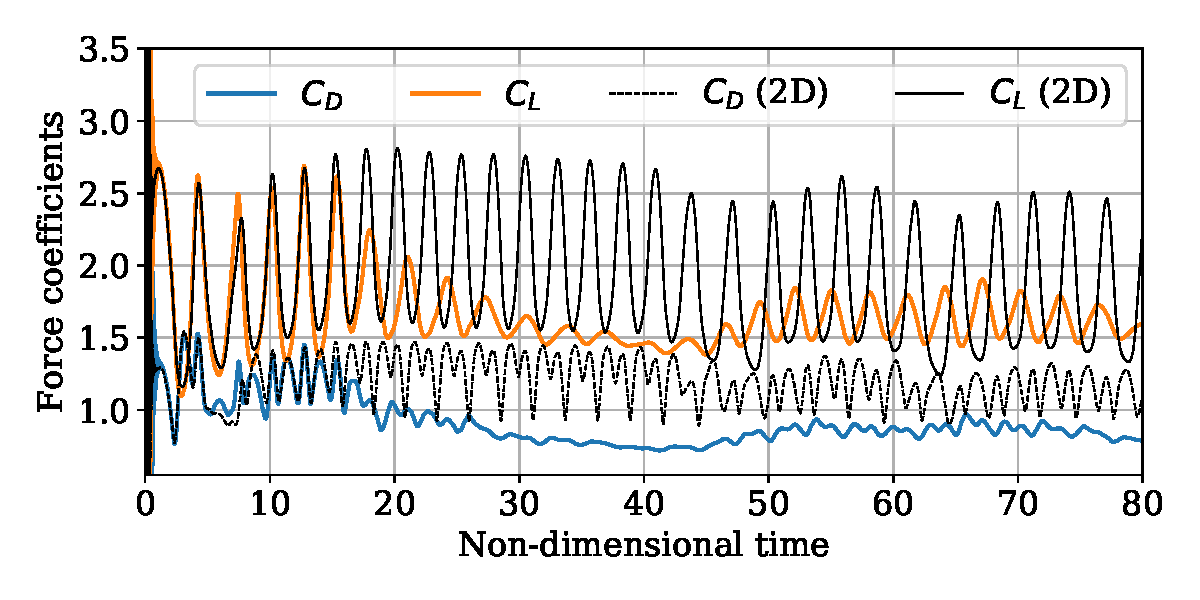
\includegraphics[width=8cm]{figures/forceCoefficientsCompare2D.pdf}
    \caption{History of the force coefficients obtained with two- and three-dimensional simulations at Reynolds number $2000$ for a snake cross-section with a $35$-degree angle of attack.}
    \label{fig:force_coefficients}
\end{figure}

\begin{figure}[!h]
    \centering
    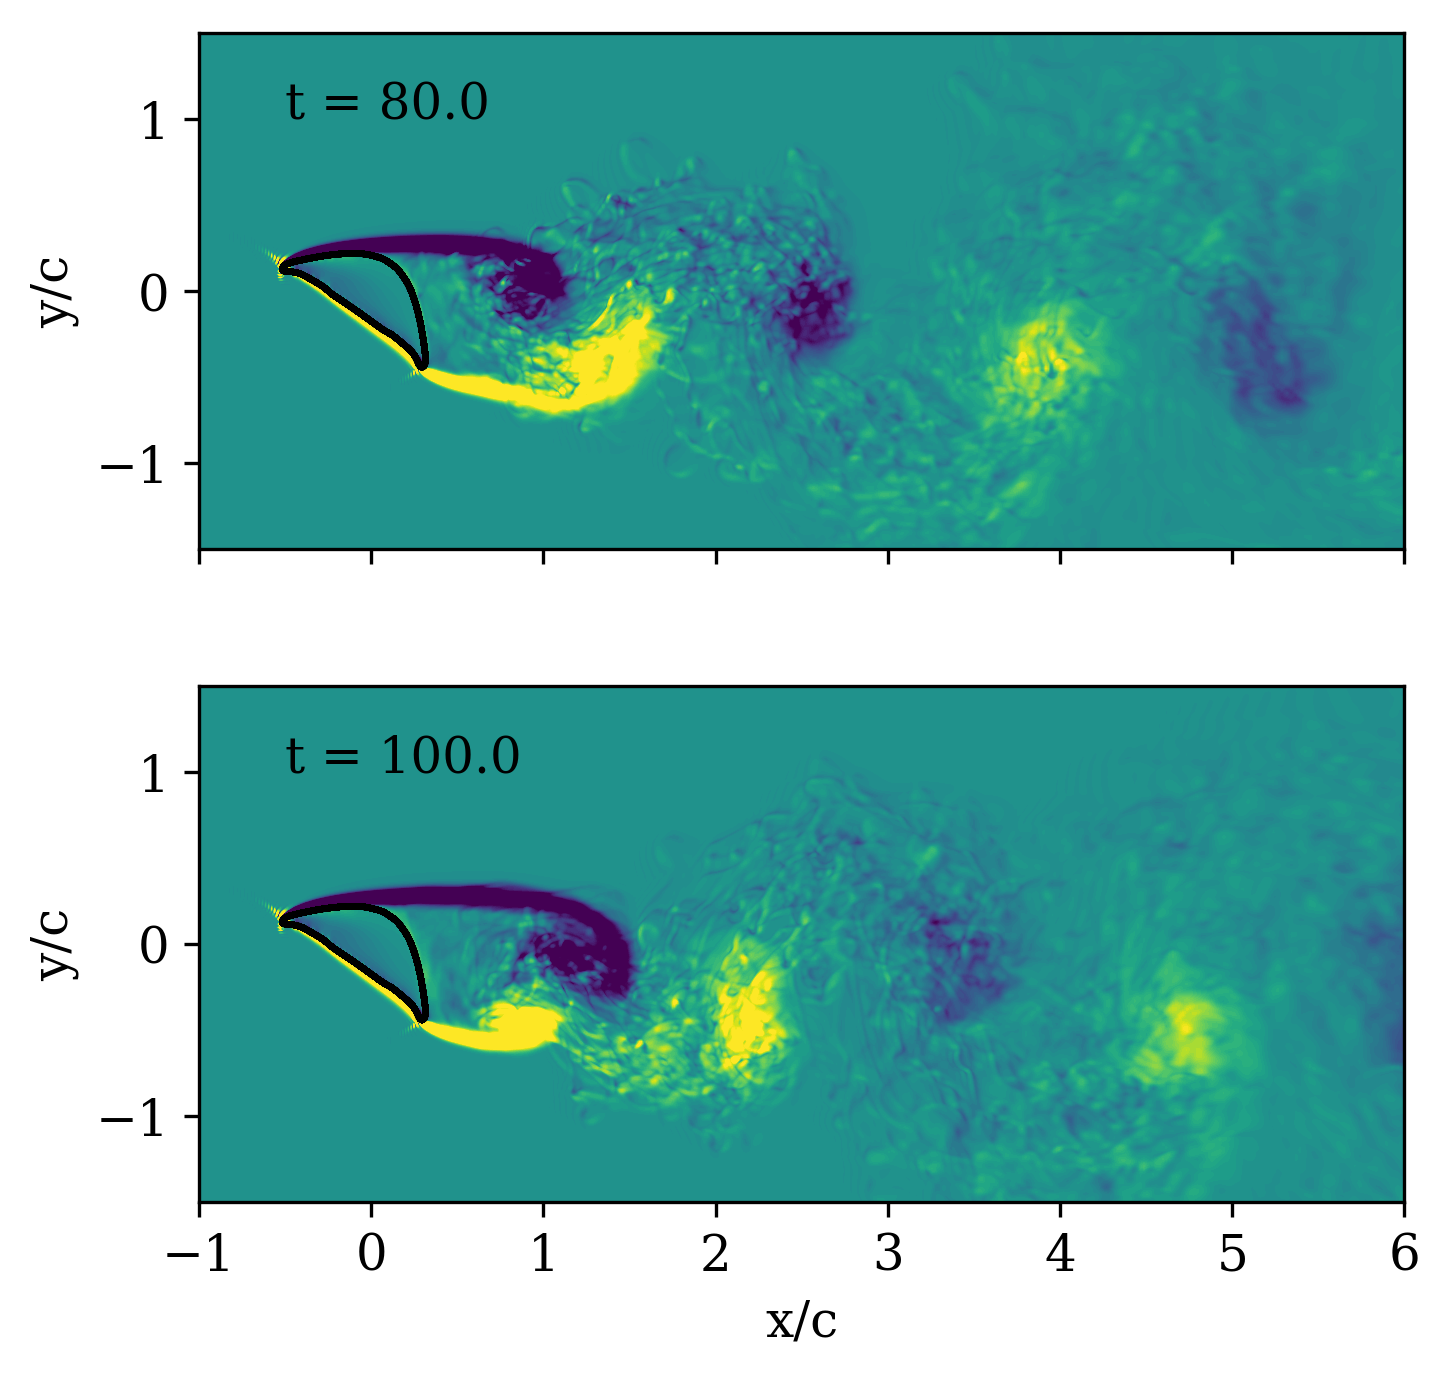
\includegraphics[width=8cm]{figures/wz_avg_multi_contourf.png}
    \caption{Filled contour of the spanwise-averaged z-component of the vorticity ($-5 \leq w_z c / U_\infty \leq 5$) field after $80$ and $100$ time units of flow simulation with PetIBM for the snake cylinder with a cross-section at a $35$-degree angle of attack and Reynolds number $2000$.}
    \label{fig:wz_avg_3d}
\end{figure}

\begin{table}[!h]
    \caption{Time-averaged force coefficients on the snake cross-section at Reynolds number 1000 and angle of attack $35^o$ for the two- and three-dimensional configurations. (We average the force coefficients between $40$ and $80$ time units of flow simulation.)}
    \label{tab:force_coefficients}
    \centering
    \begin{tabular}{ccll}
        \hline
        Case & Mesh size & $<C_D>$ & $<C_L>$ \\
        \hline
        3D & $1071 \times 1072 \times 40$ & $0.8390$ & $1.5972$ \\
        2D & $1704 \times 1706$ & $1.1567$ ($+37.9\%$) & $1.8279$ ($+14.4\%$) \\
        \hline
    \end{tabular}
\end{table}

\section{Cost Analysis}\label{sec:cost}

% \section*{Acknowledgment}

\bibliographystyle{IEEEtran}
% argument is your BibTeX string definitions and bibliography database(s)
\bibliography{IEEEabrv,MesnardoBarba2019}
%
% <OR> manually copy in the resultant .bbl file
%\begin{thebibliography}{1}
%\bibitem
%\end{thebibliography}

\end{document}


